\chapter{Los algoritmos evolutivos multiobjetivo}\label{ch:multiobj}

El tipo de algoritmos al que pertenecen aquellos que serán estudiados e implementados en este trabajo son los llamados algoritmos evolutivos multiobjetivo. Para comprenderlos bien, primero será necesario estudiar los dos conceptos clave en los que se basan: la optimización multiobjetivo y los algoritmos evolutivos.

\section{Optimización multiobjetivo}

Antes de comenzar a definir la optimización multiobjetivo, para situar al lector sería lógico hablar brevemente sobre la optimización clásica, es decir, aquella cuyo objetivo consiste en optimizar una única funcion. Eso es justamente lo que se hará a continuación.

\subsection{Problema de optimización de un objetivo}

En los problemas de optimización convencionales, el objetivo consiste en encontrar una solución, dentro del espacio de soluciones posibles, que optimice una única función objetivo. Ya se vio un ejemplo en la sección \ref{subsct:optclust} , donde se formula sin mucho rigor el problema del clustering como un problema de optimización. Una definición general y más formal de los problemas de optimización sería la siguiente:

\begin{definicion}
	
	\emph{\textbf{Problema General de Optimización de un Único Objetivo}:} Un problema de optimización de un único objetivo consiste en minimizar (o maximizar) una función $f(\textbf{x})$ sujeta a $g_i(\textbf{x}) \leq 0$, $i = \{1, \dots, r\}$ y $h_j(\textbf{x})$, $j = \{ 1, \dots, p\}$. Una solución $\textbf{x}$ minimiza (o maximiza) el escalar $f(\textbf{x})$, donde $\textbf{x} \in \Omega$ es un vector $n$-dimensional de variables de decisión $\textbf{x} = (x_1,\dots,x_n)$ de un universo $\Omega$ \cite{coello2007evolutionary}. 
	
\end{definicion}

	
Como se puede ver, $g_i(\textbf{x}) \leq 0$ y $h_j(\textbf{x}) = 0$ representan restricciones que deben cumplirse al optimizar $f(\textbf{x})$. Por su parte el \emph{universo} $\Omega$ es el conjunto que contiene todas las posibles soluciones $\textbf{x}$ que pueden usarse para tanto la función objetivo $f(\textbf{x})$  como las restricciones.
	
El método por el cual se encuentra el óptimo global de una función cualquiera se llama \emph{optimización global}: 
	
\begin{definicion}
 \emph{\textbf{Optimización del Mínimo Global}:} Dada una función $f:\Omega \subseteq \mathbb{R}^n \rightarrow \mathbb{R}$, $\Omega \neq \emptyset$, para $\textbf{x} \in \Omega$ el valor $f^* \equiv f(\textbf{x}^*)$ es el mínimo global si y solo si
 \begin{equation}
 	\forall \textbf{x} \in \Omega:~~f(\textbf{x}^*) \leq f(\textbf{x}),
 \end{equation}
 
 donde $\textbf{x}^*$ es la solución mínima global, $f$ es la función objetivo, y el conjunto $\Omega$ es la región factible de $\textbf{x}$. El objetivo de encontrar la solución o soluciones mínimas globales se llama \textbf{problema de optimización global} \cite{coello2007evolutionary}.
\end{definicion}	



\subsection{Problema de optimización multiobjetivo}\label{sec:mop}

En un principio, puede parecer que la única novedad existente en la optimización multiobjetivo con respecto a la optimización convencional consiste, como su nombre indica, en la optimización de varias una funciones objetivo. Sin embargo, esta diferencia tiene implicaciones que cambian notablemente la forma en la que se trabaja en los problemas de optimización.

La optimización multiobjetivo en general puede definirse de la siguiente forma:

\begin{definicion}
	
	\emph{\textbf{Problema General de Optimización  Multiobjetivo} :} Un problema de optimización multiobjetivo consiste en minimizar (o maximizar) $F(\textbf{x}) = (f_1(\textbf{x}),\dots,f_m(\textbf{x}))$ sujeto a $g_i(\textbf{x}) \leq 0$, $i = \{1, \dots, r\}$ y $h_j(\textbf{x})$, $j = \{ 1, \dots, p\}$. Un problema de optimización minimiza (o maximiza) los componentes de un vector $F(\textbf{x}) \in \mathbb{R}^m$ donde $\textbf{x} \in \Omega$ es un vector de $n$ variables de decisión $\textbf{x} = (x_1, \dots, x_n)$ de un universo $\Omega$ \cite{coello2007evolutionary}.
\end{definicion}

De nuevo, $g_i(\textbf{x}) \leq 0$ y $h_j(\textbf{x}) = 0$ representan las restricciones, y $\Omega$ representa el espacio de soluciones o región factible.

Al optimizar más de una función objetivo, surge un nuevo problema que no se daba cuando se trabaja con una única función objetivo: que no existe una definición consensuada de qué se considera una solución óptima, por lo que resulta difícil comparar unas soluciones con otras \cite{mukhopadhyay2013survey}.


Al ser las funciones objetivo independientes entre ellas, existiendo en ocasiones incluso contradicciones entre ellas, no es posible encontrar siempre una única solución que sea óptima para todas las funciones objetivo a la vez, y por tanto no existe un orden total en el espacio objetivo, sino tan solo un orden parcial \cite{miettinen2012nonlinear}. Por ejemplo, para un espacio objetivo en $\mathbb{R}^2$, podríamos decir que el punto $(1,2)$ es menor que el punto $(3,6)$. Sin embargo, los puntos $(1,3)$ y $(2,1)$ no se podrían comparar tan fácilmente.

Es necesario establecer una forma de determinar qué soluciones son, de alguna forma, mejores que otras. Para ello, introduciremos la terminología de Pareto, que será la que nos permita comparar vectores de valores objetivo $F(\textbf{x})$ y determinar qué soluciones $\textbf{x}$ obtenidas pueden ser útiles, interesantes o válidas para el problema a resolver.

El primer concepto a definir es el de \emph{dominancia de Pareto} o \emph{Pareto-dominancia}, que nos permitirá definir una relación de orden (parcial) entre vectores de valores objetivo:

\begin{definicion}
	\textbf{\emph{Pareto-dominancia}}: un vector $\textbf{u}$ domina al vector $\textbf{v}$ (denotado $\textbf{u} \preceq \textbf{v}$) si, en caso de estar ante un problema de  minimización, $\textbf{u}$ es parcialmente menor que $\textbf{v}$ \cite{jose2016automatic}\cite{coello2007evolutionary}:
	\begin{equation}
	\textbf{u} \preceq \textbf{v} ~\Longleftrightarrow~ \forall i \in \{1,\dots,m\}:~ u_i \leq v_i ~\land~ \exists j \in \{1,\dots,m\}:~ u_j < v_j~.
	\end{equation}
\end{definicion}

Dicho en un lenguaje más natural: el vector $\textbf{u}$ domina al vector $\textbf{v}$ si todos los elementos de $\textbf{u}$ son menores o iguales a los respectivos elementos de $\textbf{v}$, y al menos uno de los elementos de $\textbf{u}$ es estrictamente menor que el elemento correspondiente de $\textbf{v}$. Nótese que esta definición asume que el problema es de minimización. Para los problemas de maximización, bastaría con cambiar los menores o iguales y los menores estrictos, por mayores o iguales y mayores estrictos, respectivamente.

A partir de la dominancia de Pareto, se definen los conceptos de \emph{optimalidad de Pareto} y \emph{conjunto de Pareto}:
\begin{definicion}
	\emph{\textbf{Optimalidad de Pareto} }: Una solución $\textbf{x} \in \Omega$ se dice que es Pareto-óptima con respecto a $\Omega$ si y solo si no existe ninguna otra solución $\textbf{x}'$ tal que $F(\textbf{x}') \preceq F(\textbf{x})$ \cite{coello2007evolutionary} \cite{miettinen2012nonlinear}.
\end{definicion}

\begin{definicion}
	\emph{\textbf{Conjunto Óptimo de Pareto}}:
: Dadas unas funciones objetivo $F(\textbf{x})$, el Conjunto Óptimo de Pareto $\mathcal{P}^*$ se compone de todas las soluciones Pareto-óptimas, es decir, todas las soluciones no dominadas del espacio de soluciones  \cite{coello2007evolutionary}:
	\begin{equation}
		\mathcal{P}^* := \{\textbf{x} \in \Omega ~|~ \neg \exists \textbf{x}' \in \Omega:~F(\textbf{x}') \preceq F(\textbf{x}) \}~.
	\end{equation}
\end{definicion}

El conjunto óptimo de Pareto está formado, en teoría, por las mejores soluciones posibles. Nótese que es todo un \emph{conjunto} de soluciones, y no una única solución óptima. Bien es cierto que, en optimización de un objetivo, pueden obtenerse más de una solución óptima para un problema determinado, pero eso significaría que sus correspondientes valores objetivos $f(\textbf{x})$ serían el mismo. En cambio, en el ámbito de la optimización multiobjetivo se da la particularidad de que se obtienen diversas soluciones óptimas (o en este caso, no dominadas) cuyos respectivos vectores de valores objetivo $F(\textbf{x})$ pueden ser distintos entre ellos, siempre y cuando ninguno de esos vectores domine a otro. Esto pone de manifiesto la complejidad adicional que supone trabajar con más de una función objetivo.

El último concepto relativo a la optimización multiobjetivo que introduciremos es el de \emph{frente de Pareto}:


\begin{definicion}
	\emph{\textbf{Frente de Pareto} \cite{coello2007evolutionary}}: dados unas funciones objetivo $F(\textbf{x})$ y un Conjunto Óptimo de Pareto $\mathcal{P}^*$, el Frente de Pareto $\mathcal{PF}^*$ se define como:
	\begin{equation}
		\mathcal{PF}^* := \{ F(\textbf{x}) ~|~ \textbf{x} \in \mathcal{P}^*\}~.
	\end{equation}
\end{definicion}

El frente de Pareto de un conjunto óptimo $\mathcal{P}^*$ no es sino la imagen del conjunto $\mathcal{P}^*$ en el espacio de valores objetivo, o lo que es lo mismo, es el conjunto de correspondientes vectores objetivo de las soluciones que componen $\mathcal{P}^*$.

¿Cómo puede obtenerse el conjunto óptimo $\mathcal{P}^*$? Un posible método consistiría en generar todas las posibles soluciones de $\Omega$, obtener los vectores de valores objetivos de estas y comprobar cuáles de ellas no son dominadas. Este método, no obstante, no es viable debido al alto número de soluciones del que normalmente se compone $\Omega$ (de hecho, incluso puede tratarse de un conjunto infinito). Como tampoco es fácil, por no decir imposible, obtener una expresión analítica para el frente de Pareto, el procedimiento normal para generarlo consiste en obtener un subconjunto de soluciones de $\Omega$ lo suficientemente grande, para posteriormente obtener sus vectores de valores objetivo y comprobar cuáles de ellos no son dominados \cite{coello2007evolutionary}.

\begin{figure}
	\centering
	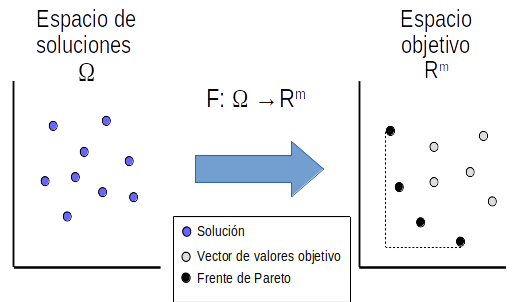
\includegraphics[width=0.9\textwidth]{Images/pareto}
	\caption{Representación gráfica de un frente de Pareto}
	\label{fig:pareto}
\end{figure}

¿Por qué se le llama \emph{frente} al frente de Pareto? Si se dibujan en una gráfica los vectores de valores objetivo $F(\textbf{x})$ de las soluciones $\textbf{x}$ obtenidas, se puede observar que aquellos puntos $F(\textbf{x})$ correspondientes a soluciones no dominadas describen una curva que se sitúa en el límite o frontera del conjunto de puntos obtenidos, y es precisamente en esa frontera donde, en teoría, se encuentran todas las soluciones óptimas, a pesar de que a priori solo se haya generado un subconjunto de ellas. La figura \ref{fig:pareto} ilustra el concepto de frente de Pareto por medio de un sencillo ejemplo.




\section{Algoritmos evolutivos}

Antes de hablar sobre los algoritmos evolutivos multiobjetivo, es lógico dedicar un espacio a los algoritmos evolutivos en general, así como a la clase de algoritmos a los que pertenecen: las metaheurísticas.

\subsection{Metaheurísticas}

Las \emph{metaheurísticas} son una familia de algoritmos de optimización aproximada, muy útiles para resolver problemas de gran dificultad y complejidad puesto que ofrecen soluciones \emph{aceptables} o que pueden considerarse suficientemente buenas en un tiempo razonable. A diferencia de otros algoritmos de optimización, las metaheurísticas no garantizan la optimalidad de las soluciones encontradas \cite{talbi2009metaheuristics}.

Las técnicas metaheurísticas pueden dividirse entre dos grupos principales \cite{jose2016automatic} \cite{talbi2009metaheuristics}:

\begin{itemize}
	\item \textbf{Metaheurísticas de una única solución}. En este tipo de metaheurísticas, una única solución se va mejorando de acuerdo a una función objetivo, de forma que esta solución representa, en muchos casos, un punto que va siguiento una trayectoria en el espacio de soluciones. Ejemplos de esta clase de algoritmos son el enfriamiento simulado (\emph{Simulated Annealing}) \cite{kirkpatrick1983optimization} y la búsqueda tabú (\emph{Tabu Search}) \cite{glover1990tabu}.
	\item \textbf{Metaheurísticas basadas en poblaciones}. Estos algoritmos, como su propio nombre indica, trabajan con toda una población de soluciones. Dicha población es inicializada aleatoriamente, e iterativamente se van generando nuevas poblaciones que son de alguna forma integradas en la población principal usando un cierto criterio de selección. La ventaja de trabajar con toda una población de soluciones en vez de con solo una de ellas es que permite diversificar el proceso de búsqueda en el espacio de soluciones. Ejemplos de metaheurísticas basadas en poblaciones son los algoritmos genéticos o GA (\emph{Genetic Algorithms}) \cite{holland1992adaptation}, la evolución diferencial o DE (\emph{Differential Evolution}) \cite{storn1997differential}, la optimización por nube/enjambre de partículas o PSO (\emph{Particle Swarm Optimization}) \cite{kennedy1995particle} y la optimización por colonia de hormigas o ACO (\emph{Ant Colony Optimization}) \cite{dorigo1996ant}.
\end{itemize}

A su vez, dentro de las metaheurísticas basadas en poblaciones se encuentran los llamados \emph{algoritmos evolutivos}, al que pertenecen, entre otros, los algoritmos genéticos y las técnicas de evolución diferencial.

\subsection{Conceptos básicos de los algoritmos evolutivos}

Los algoritmos evolutivos o EAs (\emph{Evolutionary Algorithms}) tienen en común el hecho de que se basan en la evolución biológica de las especies, de forma que a los individuos de la población de les aplican operadores evolutivos para generar nuevos individuos (llamados \emph{descendientes}) a partir de ellos.
 
Un \emph{individuo} representa una solución codificada al problema que se pretende optimizar, y suele estar representado por cadenas o secuencias de valores, que corresponden al \emph{genotipo} en términos biológicos. El genotipo de un individuo se compone de un cromosoma (o más), y a su vez un \emph{cromosoma} se compone de genes que pueden adoptar determinados valores (\emph{alelos}). De esta forma, cada individuo codifica una serie de parámetros usados como valores de entrada de la función que se desea optimizar. Por último, un conjunto de cromosomas se denomina \emph{población}. \cite{coello2007evolutionary}

Con el fin de generar soluciones cada vez mejores, sobre la población se aplican una serie de operadores inspirados en la biología y la selección natural, llamados \emph{operadores evolutivos}. Los tres operadores usados en los algoritmos evolutivos son: el operador de \emph{cruce} o \emph{recombinación}, el operador de \emph{mutación} y el operador de \emph{selección} \cite{coello2007evolutionary}. A grandes rasgos, el operador de cruce permite generar una o varias soluciones nuevas (descendientes) a partir de una pareja de soluciones de la población (padres). El operador de mutación, por su parte, permite introducir pequeñas alteraciones en las soluciones para, por ejemplo, hacerlas ligeramente diferentes de sus soluciones padres. Finalmente, el operador de selección se utiliza para dar, en general, mayor probabilidad de reproducirse (es decir, de usar el operador de cruce) a los individuos mejores, mientras que análogamente se da menor probabilidad a los peores individuos.

\begin{figure}[h]
	\centering
	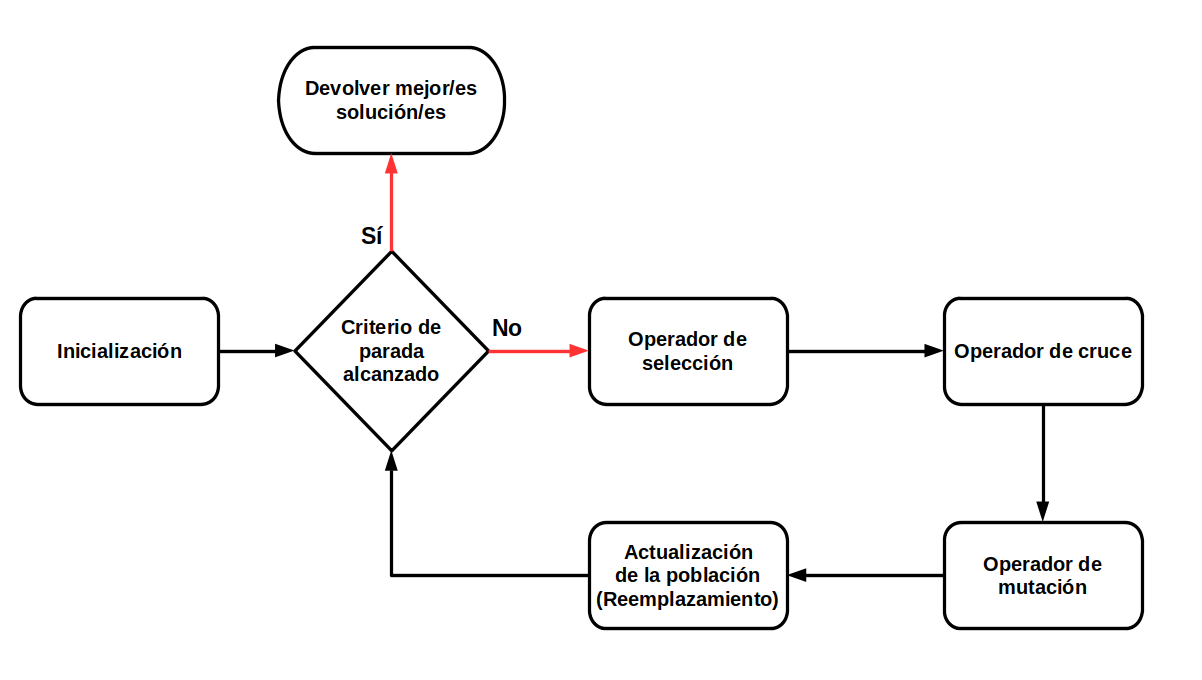
\includegraphics[width=1.0\textwidth]{Images/ga_flowchart}
	\caption[Codificación real.]{Diagrama de flujo de un algoritmo genético, un tipo de algoritmo evolutivo.}
	\label{fig:ga}
\end{figure}


Como ya se sabe, al ser los algoritmos evolutivos un tipo de algoritmos de optimización, estos trabajan con una función objetivo que se pretende optimizar, también llamada en estos casos función de \emph{fitness} \cite{coello2007evolutionary}. La función de \emph{fitness} asignan un valor numérico a las soluciones de conforman la población indicando cómo de buena es cada una de ellas, y es en este valor de bondad en el que se basa el operador de selección para asignar a cada solución su probabilidad de reproducirse.

\subsection{Algoritmos evolutivos para clustering y clustering con restricciones}\label{subsct:evolclust}

Como ya se vió en la sección \ref{subsct:optclust}, el clustering puede formularse como un problema de optimización, y como tal puede ser resuelto con algoritmos evolutivos. Para ello es necesario establecer dos elementos fundamentales: una función objetivo y un esquema de representación o codificación (es decir, la forma en que se codifican los cromosomas que corresponden a las distintas soluciones de la población).

En el caso del clustering clásico, cualquiera de los índices de validación expuestos en la sección \ref{subsct:cvi} puede usarse como función objetivo, mientras que para el clustering con restricciones podría (o debería) usarse un índice o función que tenga en cuenta de alguna forma las restricciones que han sido satisfechas o no. Lo que sí pueden usarse de la misma forma para ambos problemas son los esquemas de representación. Los esquemas de representación para el clustering (y el clustering con restricciones) pueden agruparse en tres clases \cite{jose2016automatic}:

\begin{itemize}
	\item \textbf{Codificación binaria}: Una solución se representa con una secuencia de $N$ dígitos binarios, donde $N=|\textbf{X}|$ es el número de objetos en el conjunto de datos, de forma que cada posición corresponde a un objeto del conjunto de datos. El valor de la $i$-ésima posición será igual a $1$ si el $i$-ésimo objeto del conjunto de datos corresponde a un centroide o prototipo de cluster, mientras que será igual a $0$ en caso contrario.
	
	\begin{figure}[h]
	\centering
	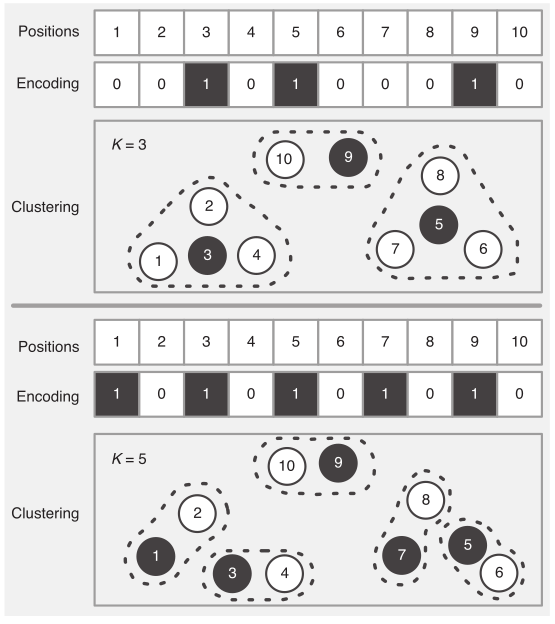
\includegraphics[width=0.8\textwidth]{Images/binary}
	\caption[Codificación binaria para $K=3$ y $K=5$ clusters.]{Codificación binaria para $K=3$ y $K=5$ clusters \cite{jose2016automatic}.}
	\label{fig:binaryencod}
\end{figure}
	
	\item \textbf{Codificación entera}: De forma similar a la codificación binaria, las soluciones se representan con secuencias de $N$ números enteros que codifican todos los objetos del dataset. A su vez, existen dos tipos de esquemas de representación con números enteros:
	\begin{itemize}
		\item \textbf{Representación basada en etiquetas}: En cada posición se guarda un valor entero del conjunto $\{1, \dots, K_{max} \}$ (o del conjunto $\{0, \dots, K_{max}-1 \}$ si se empieza desde el $0$), donde $K_{max}$ es el número máximo de clusters que pueden formarse. De esta forma, si en la posición $i$ del cromosoma aparece el valor $k$, significa que el $i$-ésimo objeto del conjunto de datos $x_i$ pertenece o ha sido asignado al cluster $c_k$.
		
		\begin{figure}[h]
	\centering
	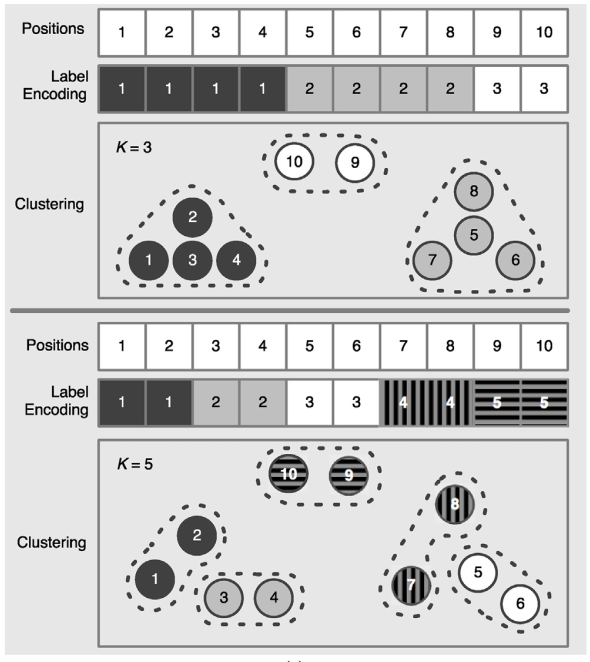
\includegraphics[width=0.8\textwidth]{Images/labelbased}
	\caption[Codificación entera basada en etiquetas.]{Codificación entera basada en etiquetas \cite{jose2016automatic}.}
	\label{fig:labelbasedencod}
\end{figure}
		
		\item \textbf{Representación basada en grafos}: En este esquema el conjunto de datos es tratado como un grafo dirigido. Cada posición de la secuencia puede almacenar valores enteros del conjunto $\{1, \dots, N \}$ (o $\{0, \dots, N-1 \}$), de forma que si en la posición $i$ aparece el valor entero $j$, esto quiere decir que el objeto $x_i$ está conectado al objeto $x_j$. De esta forma, la solución de clustering se construye identificando las distintas partes conexas del grafo, de forma que cada parte conexa del grafo corresponde a un cluster.
	\end{itemize}
	


	\begin{figure}[h]
	\centering
	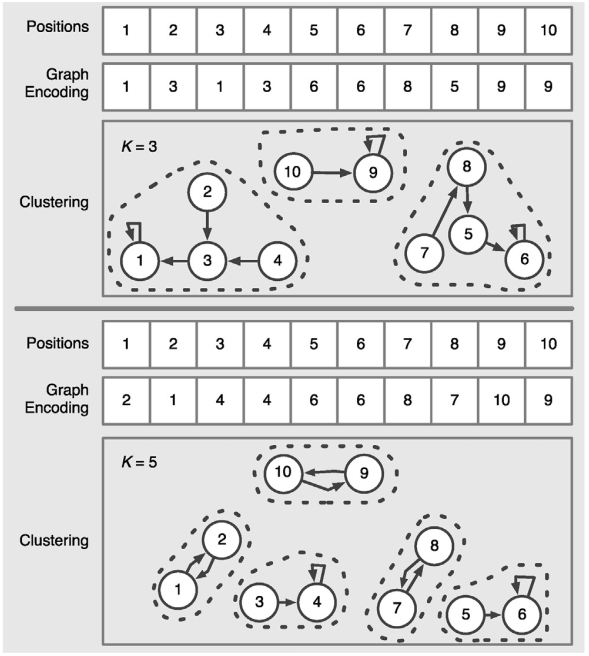
\includegraphics[width=0.8\textwidth]{Images/graphbased}
	\caption[Codificación entera basada en grafos.]{Codificación entera basada en grafos \cite{jose2016automatic}.}
	\label{fig:graphbasedencod}
\end{figure}
	
	\item \textbf{Codificación real}: En este tipo de codificación, los cromosomas representan las localizaciones o coordenadas de los centroides de los clusters en el espacio de características de $D$ dimensiones. Si en el problema a resolver existen $N$ objetos en un espacio $D$-dimensional, los cuales deben ser agrupados en $K$ clusters, entonces los centroides de una solución determinada pueden codificarse con matrices de $D \times K$ valores reales. La codificación real puede ser de tamaño fijo o tamaño variable:
	\begin{itemize}
		\item \textbf{Codificación de longitud fija}: Las soluciones se codifican asumiendo un predeterminado número máximo de clusters $K_{max}$, de forma que todos los cromosomas de la población mantienen la misma longitud de $D \times K_{max}$. Junto a los cromosomas suelen usarse vectores con umbrales de activación para determinar cuáles de esos $K_{max}$ clusters están participando realmente en el agrupamiento.
		
		\item \textbf{Codificación de longitud variable}: Si se tiene un conjunto de $P$ soluciones $\mathcal{C} = \{\textbf{C}_i ~|~ i = 1, \dots, P \}$, la $i$-ésima solución codifica un cierto número de centroides $K_i$. Por tanto, la longitud del cromosoma será variable dependiendo de la solución, teniendo un tamaño de $D × K_i$, aspecto que debe ser tenido en cuenta al hacer uso de los operadores evolutivos.
	\end{itemize}	
\end{itemize}

\begin{figure}
	\centering
	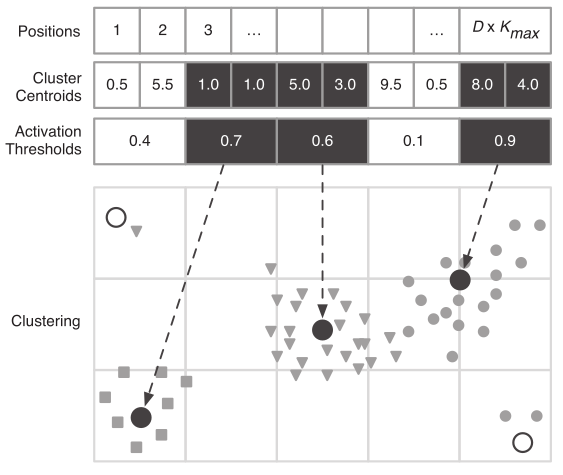
\includegraphics[width=0.8\textwidth]{Images/real}
	\caption[Codificación real.]{Codificación real \cite{jose2016automatic}.}
	\label{fig:realencod}
\end{figure}




Existen diversos ejemplos del uso de algoritmos evolutivos para el problema del clustering y del clustering con restricciones. En \cite{sheikh2008genetic}, por ejemplo, se realiza un análisis sobre el uso de técnicas de clustering basadas en algoritmos genéticos. Por otra parte, en \cite{gonzalez2020dils} se propone un algoritmo evolutivo con búsqueda local, al que llaman DILS (\emph{Dual Iterative Local Search}), en cuya función de \emph{fitness} se suma, por un lado, la sumatoria de distancias al cuadrado entre elementos del mismo cluster, y por otro, un factor de penalización que aumenta cuantas más restricciones son violadas (o sea, no satisfechas). Se trata, como es lógico, de una función de minimización, puesto que una solución es mejor cuanto más cercanos sean los elementos de un mismo cluster y cuantas más restricciones satisfaga.


En definitiva, el uso de algoritmos evolutivos en problemas de clustering, con o sin restricciones, es idóneo dados, por un lado, el hecho de que encontrar la partición óptima en un problema del clustering es de una alta complejidad, y por otro, el hecho de que los algoritmos evolutivos ofrezcan soluciones lo suficientemente buenas en un tiempo aceptable.

\section{Algoritmos evolutivos multiobjetivo}

Los algoritmos evolutivos multiobjetivo o MOEAs (\emph{Multi-Objective Evolutionary Algorithms}) son especialmente adecuados para los problemas de optimización multiobjetivo, ya que al ser algoritmos basados en poblaciones están diseñados para manejar múltiples soluciones durante el proceso de búsqueda \cite{mukhopadhyay2013survey}. 

Una característica relativa a la terminología de Pareto que distingue a los MOEAs de los EAs es el uso de poblaciones adicionales de individuos que no son Pareto-dominados. Muchos MOEAs manejan una población secundaria de soluciones, que al principio está vacía, en la que se van almacenando todas las soluciones no dominadas que se han encontrado hasta el momento. Como la Pareto-dominancia de un vector depende del contexto en el que es evaluado, cada vez que se añade una solución o conjunto de soluciones no dominadas a esa población, las soluciones ya incluidas deben ser comprobadas para asegurarse de que siguen siendo no dominadas. De lo contrario, dichas soluciones son eliminadas de la población secundaria \cite{coello2007evolutionary}.

Tipos de MOEAs

\begin{itemize}
\item A Priori
\item Progresivos
\item Posteriori
\end{itemize}

(Ejemplos de MOEAs)

Uso de MOEAs para clustering (¿clustering con restricciones?)

La ventaja de usar MOEAs para resolver problemas de clustering clásico, al ser multiobjetivos, permiten usar múltiples índices de validación. Pueden usarse al mismo tiempo tanto índices que priorícen la cohesión intra-cluster (p.ej.: minimizar distancias entre las instancias y los centroides de los clusters a los que pertenecen, minimizar distancias entre instancias del mismo cluster, etc.) como índices que se enfoquen en la distancia entre clusters (p.ej.: maximizar distancias entre centroides de los clusters, maximizar distancias entre instancias de clusters distintos), sin que se establezca un orden de prioridad entre ellas.

Además, los MOEAs también son especialmente idóneos para ser usados con problemas de clustering con restricciones, ya que permiten usar como funciones distintas e independientes, por un lado, los índices de validación para clustering clásico para evaluar la calidad de la agrupación obtenida, y por otro, alguna función de insatisfacibilidad para controlar en qué grado se respetan las restricciones impuestas.


